\documentclass[runningheads]{llncs}
\usepackage{amssymb}
\setcounter{tocdepth}{3}
\usepackage{graphicx,epsfig}
\usepackage{algorithmic}
\usepackage{listings}
\usepackage{rotating}
\usepackage{subfig}

%%%%

\usepackage{color}
\usepackage{alltt}
\usepackage{verbatim}
\usepackage{url}
\usepackage[latin1]{inputenc}
%\usepackage[spanish]{babel}


%%
%COSAS A CAMBIAR (FERGU)
% Quitar todos los "it's" mal puestos
% Poner bien las comillas, así: ``yeja''
% No hablar de los logs y las cosas técnicas que permitan integración (o sea, poca ingeniería). Lo de las expresiones regulares tampoco nos interesa demasiado, lo importante son los resultados
% Sí, da las gracias a la fundación al final (pero ahora es anónimo!)
% Si es para EvoGames no podemos decir literario, y viceversa (tendríamos que quitar lo de Skyrim por ejemplo)
% Enlazar mejor lo de antes de "In this work, several..."
% Sí que creo que habría que decir las características que tiene un perfil, nombrarlas al menos o decir su número (para saber el tamaño de los individuos del EA).
% Quitar la figura lifecyle y decir que no nos cabe, pero que se puede bajar del github. Demasiada información y no se va a ver...
% shows the average of the best fitness and the average of the average fitness for 30 executions ---> shows the average of the best fitness and the average population fitness at the end of each execution
% Results for 30 executions of each configuration for 1 to 5 profiles --> using 1 to 5 profiles.
% Decir en algún lado, que el tamaño del individuo entonces también varía (no es lo mismo un individuo de 1 perfil que tendrá 12 parámetros que uno de 5 que tendrá 60)
% set-up -> setup
%  Hay que dejar claro que es cada cosa: perfil y características y seguir la misma nomenclatura para que la gente no se pierda. Aquí el ejemplo: The MADE Agent is created using 12 parameters --> ... using 12 parameters, that is, its profile.
% Hay que poner una gráfica de cómo va la evolución del fitness con 1..5 perfiles


\usepackage{url}
\urldef{\mailsa}\path|rhgarcia@fidesol.org|
\urldef{\mailsb}\path|pgarcia@atc.ugr.es|
\urldef{\mailsc}\path|jmerelo@geneura.ugr.es|



\newcommand{\keywords}[1]{\par\addvspace\baselineskip
\noindent\keywordname\enspace\ignorespaces#1}

\lstset{
basicstyle=\ttfamily \scriptsize,
language=c++,
frame=single,
stringstyle=\ttfamily,
showstringspaces=false
}

\begin{document}
 %\pagestyle{empty} %ESTO QUITA LOS NUMEROS DE PAGINA
\mainmatter  % start of an individual contribution



% first the title is needed

% (Rubén): Cambio el título de "MADE: A Massive Artificial Drama Engine for non-player characters"
% a "Emerging archetypes in massive Artificial Societies for literary purposes using Genetic Algorithms"
% porque me parece más fiel al contenido del artículo

\title{Emerging archetypes in massive Artificial Societies for literary purposes using Genetic Algorithms}


% a short form should be given in case it is too long for the running head
\titlerunning{Emerging archetypes in massive Artificial Societies for literary purposes}
%\author{R.H. Garc\'ia-Ortega\inst{1}, P. Garc\'ia-S\'anchez\inst{2} and J.J. Merelo\inst{2}}
\author{A.U. Thor\inst{1}}
%

%\authorrunning{R.H. Garc\'ia-Ortega et al.} 
% (FERGU): OJO! ES DOBLE CIEGO
% (Rubén): ¿Y cuando es doble ciego, qué se hace con el autor? ¿lo dejo así?

% (feature abused for this document to repeat the title also on left hand pages)
% the affiliations are given next; don't give your e-mail address
% unless you accept that it will be published

%\institute{Fundaci\'on I+D del Software Libre, Granada, Spain \and Dept. of Computer Architecture and Technology, University of Granada, Spain 
%\mailsa, \mailsb, \mailsc\\}
\institute{Anonymous institute}


% (Rubén): Esto de los tocs no se de que va

\maketitle


% -----------------------------------------------------------------------------
% ABSTRACT


\begin{abstract}

% (JJ): Es mejor que empecéis por escribir el abstract, qué es lo que queréis
% hacer, porque todo el paper va a girar alrededor de eso. Siempre se
% puede modificar luego si no sale del todo bien, pero lo importante es
% tenerlo como referencia.

% (Ruben): OK, hecho.
% Estructura actual del abstract:
% 1.- Hacer historias es muy complicado
% 2.- Entorno MADE: Cientos de personajes interactuando que permiten estudiar
%     los comportamientos
% 3.- Estudio de la parametrización y número de perfiles en el Entorno MADE 
%     para crear dos grupos de arquetipos: Control de natalidad y venganza
% 4.- Se usará un GA para encontrar la mejor solución (conjunto de parámetros)
% 5.- Se confirma la aparición de los arquetipos

The creation of fictional stories is a very complex task that usually
implies a creative process where the author has to combine characters,
conflicts and plots to create an engaging narrative. This work
presents a simulated environment with hundreds of characters that
allows the study of coherent and interesting literary archetypes (or
behaviours), plots and subplots. We will use this environment to
perform a study about the number of profiles (parameters that define
the personality of a character) needed to create two emergent groups
of archetypes: "natality control" and "revenge". A Genetic Algorithm
will be used to find the fittest number of profiles and parameter
configuration that enables the existence of the desired archetypes
(played by the characters without their express knowledge). The
results show that parametrizing this complex system is possible and
that these kind of archetypes can emerge in the given environment. 

\end{abstract}


% -----------------------------------------------------------------------------
% INTRODUCTION


\section{Introduction}
\noindent 

NPCs (Non Player Characters) In video games are a type of characters that live in the game world to provide a more inmersive experience. Modern RPGs (Role Playing Games), such as The Witcher\texttrademark or Skyrim\texttrademark count with hundreds of NPC characters. The effort to create a good interactive fiction script is directly proportional to the number of these characters. That is the reason this kind of agents usually counts with limited behaviours, such as wandering in the villages, selling groceries or guarding the cities. Also, they usually offer scripted conversations, for example, for buy and sell objects to the player. In other cases they interact with the player depending of the player's behaviour: for example, if the player steals something a city guard would attack him.  However, these characters do not interact among them, only with the player, and their activities are only guided with this purpose. In a world with such a number of characters, their collective interactions could improve the gaming experience, leading to a richer and more inmersive world. For example, hungry inhabitants could become thieves, guards could pursuit the thieves, villagers could fell in love with others or different war alliances could emerge.

These facts have motivated us to develop a multi-agent system called MADE (Massive Artificial Drama Engine) to model a self-organized virtual world where their elements influences each other, following a cause-effect behaviours in a coherent manner. This system needs to be a suitable environment for the plot of a specific literary work, being also interesting for the player/spectator. A set of probabilities and states are associated to agents' actions, and these probabilities are optimized by means of an Evolutionary Algorithm (EA) to match with a specific literary archetype, defined by the fiction creator. The archetypes are behaviours and patterns universally accepted and present in the collective imaginary \cite{ArchetypesGarry05}, that allows empathize with the characters and immerse yourself in the story (for example, the well-known ``hero'' archetype).

In this work, several experiments have been carried out to answer the following questions: 

% (JJ): No se da "insight" a una pregunta: lo dan las respuestas.
% (Rubén): cambiado a "answers"

\begin{itemize}
 \item Is it possible to model a virtual environment inhabited by hundred of characters with interesting auto-generated behaviour based on literary archetypes?
 \item Could the personality of the agents be parametrized to obtain different behaviours? 
 \item How many profiles (groups of parameters that define a personality) are necessary to generate emergent quality sub-plots?
 \item Could a Genetic Algorithm be used to find the fittest parameter values that allow the creation of this kind of sub-plots?
\end{itemize}

% (JJ): si esto es todo, es muy pobre. En un paper tienes que hacerte
% preguntas y repsonderlas. Aquí tendría que venir "in this paper we
% prove that EAs, together with the proper design of a
% (Rubén): OK, añadido un párrafo donde señalo los resultados obtenidos

In this paper we prove that EAs, together with a proper design of literary patterns, can be used to find the parameters that promote the generation of drama plots and sub-plots in a multi agent based environment.\\

The rest of the work is structured as follows: after the state of the art, the developed system is presented in Section \ref{sec:made}. Then, the experiments conduced with the EA are showed (Section \ref{experimentalsetup} \ref{sec:results}). Finally, conclusions and future works are discussed.

% -----------------------------------------------------------------------------
% SEC SOA

\section{State of the art}
\label{sec:soa}

% (JJ): Por cierto, acabo de ver esto: \cite{StoryTecGobel2008}.

Auto-generated interactive fiction research is mainly focused in methods to create the process of a story generation \cite{nairat2011character}. Story generation can be divided in two areas: interactive and non-interactive. In the first area, and according to \cite{ReviewArinbjarnar09}, an Interactive Drama is defined in a virtual world where the user has freedom to interact with the NPCs and objects in a dramatically interesting experience, different in each execution, and adapted to the interactions of the user.

% (JJ): Decir qué técnicas utiliza y qué se suele hacer en este caso


The generation of interactive dramas can also be based in script
structure \cite{ArchitectureYoung04}, where each possibility in the
story must be previously defined, so there is a limited number of
possible plot combinations. There exist other techniques, not based in
plot structure, such as... 

% (JJ): Pero esto debería ir antes de la
% descripción de MADE. Lo que digas de MADE
% al final de todo, para expresar el avance
% con respecto al estao del arte actual - JJ

% (Rubén): Done!

On the other side, in non-interactive plot generation systems the user does not take control as the protagonist. For example, in the system presented by Pizzi et al. \cite{pizzi2007interactive} the user can interact with the characters, changing their emotions, but making the user an spectator, rather as an actor.

% (FERGU): ESTO NO ME QUEDA TAMPOCO CLARO, SI NO ES INTERACTIVA COMO MODIFICAMOS LOS PERSONAJES?
% (Rubén): TODO 


As opposed to those concepts, MADE is focused in Artificial Non Interactive Drama, because its aim is the massive generation of plots for secondary characters, to provide a context for the writer and the player to perceive a virtual world as coherent, detailed and enriched. The story generation (that is, the narrative) is not addressed by MADE, but it has been studied in the systems presents in the survey by Arinbjarnar et al. in \cite{ReviewArinbjarnar09}.

% (JJ): Decir qué te hace suponer que esto va a ser una buena solución.


Previous works define the plot as an emergence for the behaviour of the agents that follow a set of rules. In MADE, the agents' behaviour is product of its personality and the environment. That is, the agents does not follow the plot, but they generate the plot itself. 

% (FERGU): ESTO NO LO TENGO MUY CLARO
% (Rubén): Así es, bien explicado.

Futhermore, the previous works generate plots in worlds with a limited number of characters. This restriction does not exist in MADE, where the number of characters to create is unlimited.


% \section{MADE} <- (Rubén) ya no es sección
% \label{sec:made} <- (Rubén) ya no es sección

% (JJ): Me parece mal comienzo... ¿Por qué sigues esas ideas, por ejemplo?
% Tendrías que haberlo dicho en la intro - JJ

% (Rubén): OK, de hecho, subo todo esto que antes se llamaba sección "MADE" a la intro.
% La siguiente sección será "The MADE Environment"

% (Rubén): TODO Explicar por qué sigo esas ideas y releer para que el texto encaje donde debe

Following the ideas of the work of Epstein and Axtell
\cite{epstein1996growing} an environment based in {\em Sugarscape} has
been developed, with concepts such as food, metabolism and
vision. This environment uses the elements  by Gershenson %nunca coma
                                %antes de verbo - JJ
\cite{gershenson2005general}: a virtual world, agents who born, grow,
interact, reproduce and dead; resources (food), mediators, and
relations of rivalry (friction) and cooperation (synergy). The actions
of these agents are parametrized according the work of Nairat
\cite{nairat2011character}, based in the existence of profiles, and
will be mapped into a chromosome to be used in a Genetic Algorithm
(GA). This system allows the definition of behaviour patterns (or
archetypes, and using a multi-objective fitness function to measure
the presence of the desired archetypes. %OJO! ESTO QUE HE DICHO ES
                                %VERDAD? (Fergu) 

% (FERGU): Comprobar que hemos mencionado en el SOA los trabajos de Epstein y Gerhenson
% (Rubén): TODO 

% -----------------------------------------------------------------------------
% SEC MADE

\section{The MADE Environment}
\label{sec:made}

The MADE enviroment is a virtual place where different agents play their artificial lives. Its functions are:

\begin{itemize}
\item \textbf{Create an initial set of agents:} MADE environment
  initializes a set of just born orphan agents, each with a profile
  sequentially assigned. % Sequentially de qu� secuencia? - JJ
 These agents must compete or collaborate in order to survive.
\item \textbf{Place agents in the map:} the environment has a squared map, formed by cells that can be occupied by one (and only one) agent. The environment allows the agents to discover and interact with other agents in the neighbourhood.
\item \textbf{Start and control the time:} after the creation of the initial set of agents, the MADE environment starts the timer, day by day until a maximum date is reached.
\item \textbf{Execute each agent during a time unit (a day):} In each iteration the list of agents is randomly reordered, and after that following the new order, each agent perform an iteration of its life-cycle, and the dead agents are removed from the grid.
\item \textbf{Perform as an external agent that changes th environment:} In each iteration in the MADE environment food rations are placed in random cells. An agent only can eat if it is over a cell with a ration, so agents could move the other forcibly.
\item \textbf{Offer services to the agents:} MADE environment allow the agents to check which closer cells have food, are occupied, who agents are in a near position or which positions can be occupied.
\item \textbf{Decide the profile of the agents:} MADE allows the existence of different agent profiles. A profile is a set of characteristics which governs the agent's behaviour.
\end{itemize}

The MADE environment can be configured by using the following parameters:

% (Rubén): TODO parámetros de un entorno MADE

\begin{itemize}
\item Number of agents initially placed.
\item Map square grid dimension.
\item Number of rations randomly placed in the grid each day.
\item Duration (in virtual days) of the  execution of the environment.
% (FERGU): \item Average NO SE QUE ES ESTO xD
% (Rubén): Normal, porque fue fallo mío incluirlo como un parámetro del entorno. Es el número de veces que se ejecuta un entorno para obtener la media del fitness (por eso de que las ejecuciones pueden ser bastante estocásticas). Quito el parámetro de esta parte.
\end{itemize}

% Usas un estilo demasiado conciso. Di qu� hace cada uno de esos
% par�metros, c�mo se meten (fichero de configuraci�n o como sea), por
% qu� se eligen esos y no otros, y los valores por defecto que has
% usado. 


\subsection{MADE Agent}
A MADE Agent lives in a MADE Environment, occupies a cell in the grid, moves around looking for food or mate and interacts with other agents.

A very simple agent has been designed for this study: a virtual rat. We have modelled 4 states for it (be alive, be hungry, look for mate and be pregnant), 7 actions (move, eat, attack, defend, escape, find mate and have offspring) and parameters that define its characteristics and probabilities to perform actions depending on the state. It's important to remark that no "feelings" and no memory have been modelled in the MADE agent.

Figure~\ref{fig:madeAgent} illustrates the nature of a MADE Agent.

\begin{figure}
\begin{center}
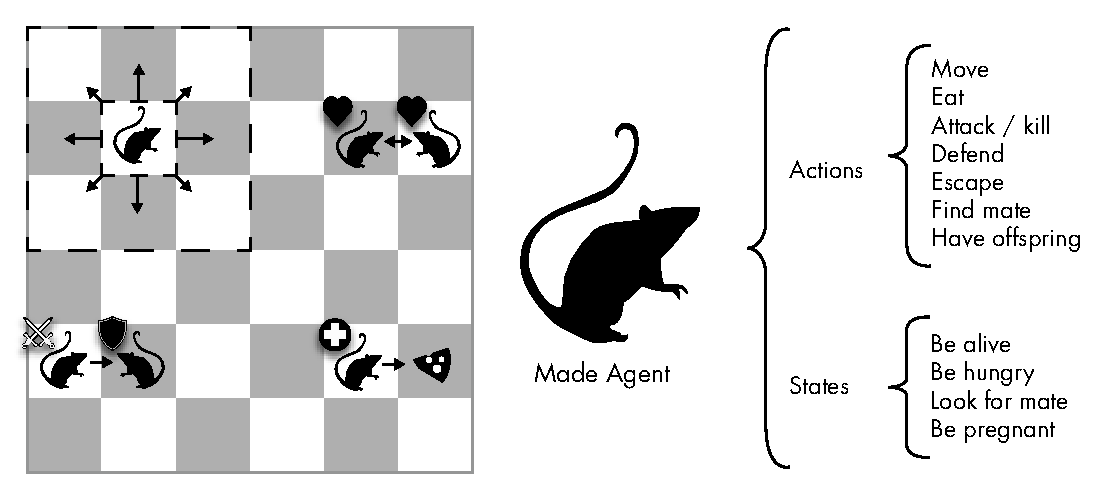
\includegraphics[scale=0.65]{img/MadeAgent.pdf}
\caption{Actions and states modelled in the MADE Agent.}
\label{fig:madeAgent}
\end{center}
\end{figure}

The life cycle of a MADE Agent illustrated in Figure~\ref{fig:life_cycle} represents on day in it's life. Every decision made by the agent is based on it's state and it's characteristics (probabilities to perform different actions).

\begin{figure}
\begin{center}
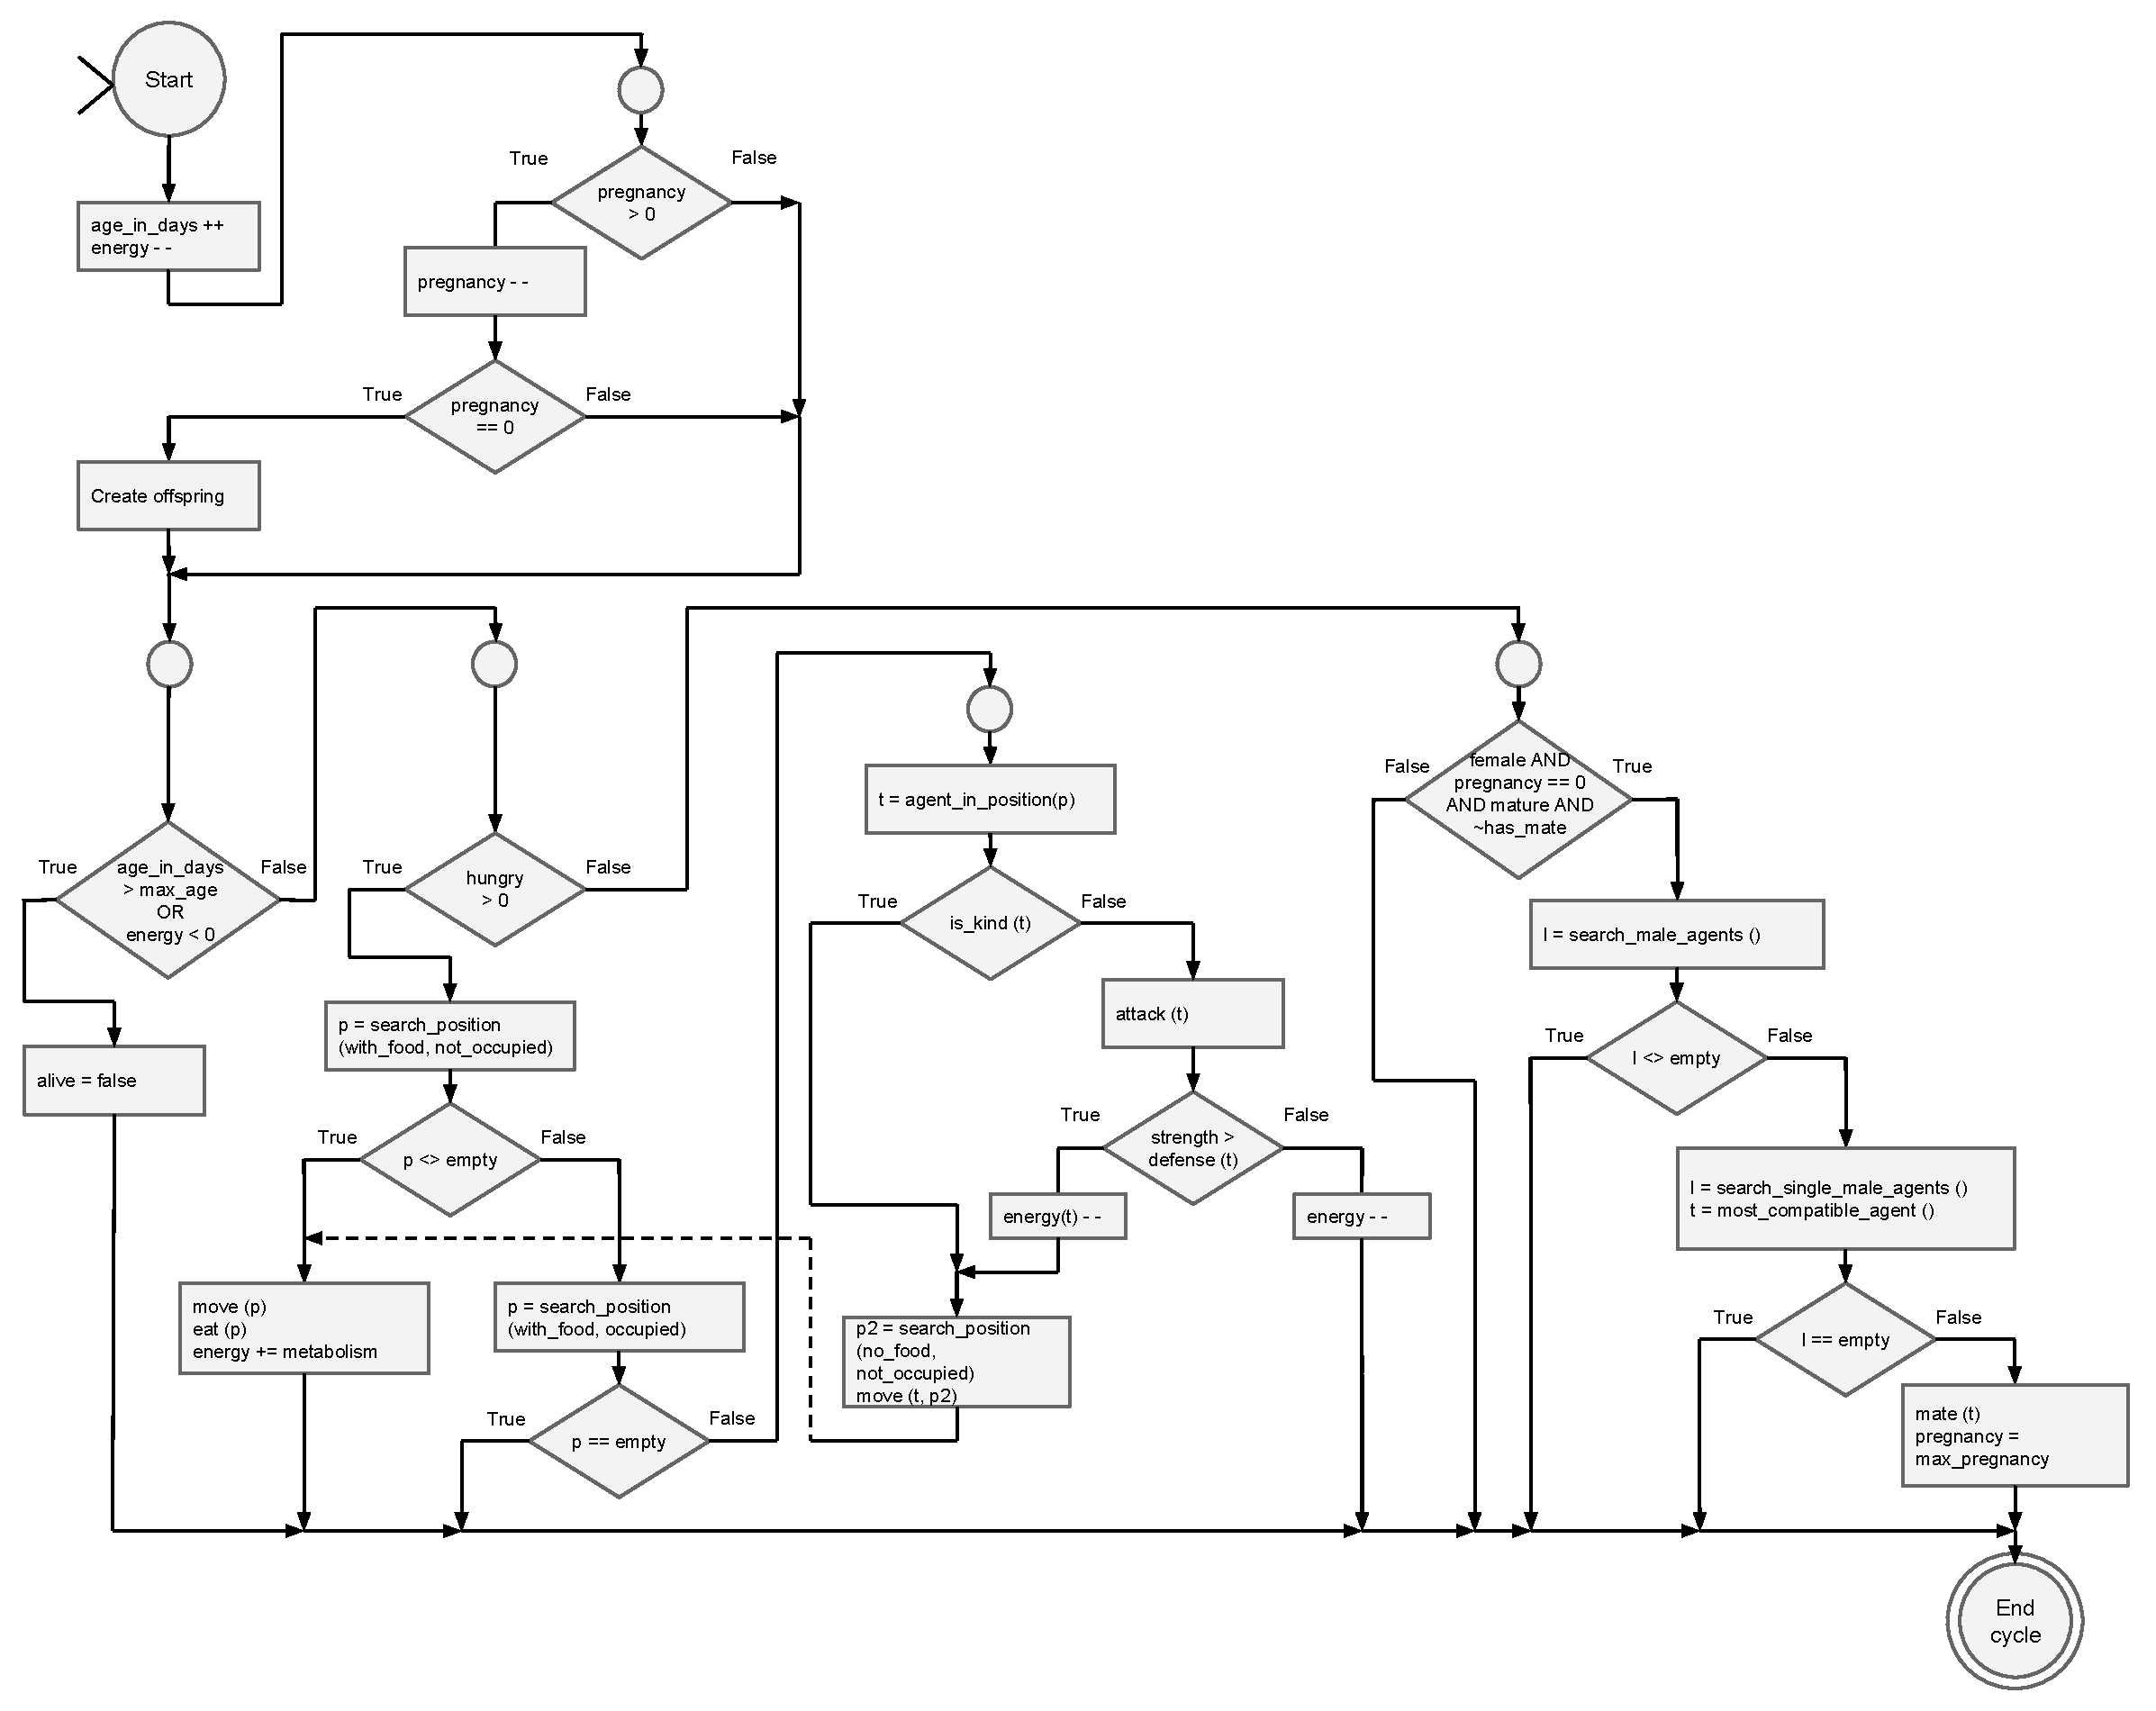
\includegraphics[scale=0.32]{img/life_cycle.pdf}
\caption{MADE Agent's life cycle}
\label{fig:life_cicle}
\end{center}
\end{figure}

% (Rubén): TODO ¿citar todas las características de un agente made?
% Sólo si hay hueco, creo
% No se ve nada y no aporta mucho. No uses notaci�n del programa, sino
% del algoritmo. Y mejor que lo contaras como un algoritmo usando el
% entorno algorithmic que este gr�fico. - JJ


\subsection{MADE Execution}

Every agent has a diary that stores all the relevant events in it's life in a simple format. Each line of the log indicates the day, the event in a short readable format and some extra information. Every agent's diary in the MADE Environment in coherent with all others' diaries. Many plots are being created, with a structured format that can be read by game engines or natural language processors, but, given the simplicity of the modelled agents, the stories could be seen by the reader as non-interesting. In the next section we propose a method based on EA to let the author of a story promote different behaviours in the MADE agents that could be seen as literary archetypes (usually associated with human feelings and high level cognitive and memory abilities).

% -----------------------------------------------------------------------------
% SEC EA
% \section{Extraction of WHATEVER using Evolutionary Algorithms}
% \label{sec:ea}
% (Rubén): Voy a hablar del uso de algoritmos evolutivos en la siguiente sección

% -----------------------------------------------------------------------------
% SEC EXPERIMENTALSETUP

\section{Experimental setup}
\label{sec:experimentalsetup}

The MADE Agent is created using 12 parameters % �has hablado antes de
                                % ellos? menci�nalo - JJ
that define its base features and probabilities to make the decisions presented in the life cycle. The execution of an agent is dynamic, and depends on the internal probabilities and states but also on the neighbourhood, and the map configuration. Even so, we can say that these initial parameters define in some way the possible situations where the agent could be involved.

Thanks to the agents' diaries, we can know every event (internal and external) of their lives, and evaluate their interest. In this work, we have implemented a method based in regular expressions with backreferences. The proposed technique puts annotations in every agent whose diary matches a complex regular expression able to find emerging high level behaviours, not implemented in the life cycle. 

In this proposal, the parameters used to define an agent will be mapped to a chromosome, and a Genetic Algorithm will be used to evolve the solution. The fitness function will be expressed in terms of:

\begin{itemize}
\item \textbf{Regular expressions applied to the diary of each agent in the environment:} An agent is tagged when a regular expression matches its diary.
% (Rubén): quitaré este: \item{A condition on the number of agents tagged:} The tag increments the fitness if the condition is true.
\item \textbf{A numeric function over the number of tagged agents for each archetype:} the fitness of the solution is increments with the returning value.
\end{itemize}

The concept of agent profile in introduced to assign different parameters to different agents. If only one profile is used, all the agents will be created with the same parameters, evolved by the Genetic Algorithm. If more profiles are used, they will be assigned to the agents in order of appearance in a loop. Our assumption is that some archetypes could emerge using one profile and other will need more (those that require two roles clearly differentiated). The more profiles are used, the harder the solution converge, since the number of alleles of the chromosome are multiplied by the number of profiles.

This work will perform a study about the number of profiles (parameters that define the personality of a character) needed to create two emergent groups of archetypes: "natality control" and "revenge".
The Genetic algorithm will use the parameters described in the Table~\ref{ga_parameters}. 

\begin{table}
\begin{center}
\caption{Parametrization of the Genetic Algorithm}
\begin{tabular}{p{3cm}p{7cm}}
\hline\noalign{\smallskip}
\noalign{\smallskip}
Parameter & Value \\
\hline
\noalign{\smallskip}
Codification & 12 alleles per profile\\
Fitness function & Average of 10 executions. Patterns are defined in sections~\ref{sec:setup_exp1} and \ref{sec:setup_exp2}\\
Natural selector & Original Rate: 0.9 \\
Crossover operator & Rate: 35\% \\
Mutation operator & Desired Rate: 12 \\
Stop condition & 100 executions\\
Generations & 30\\
Population size & 30 \\
\hline
\end{tabular}


\end{center}
\label{fig:ga_parameters}
\end{table}

%Por qu� has elegido estos experimentos y no otros? - JJ

\subsection{Experiment 1: Natality control archetype}
\label{sec:setup_exp1}

This experiment aggregates different sample archetypes where many factors must be taken into account. It will be used to answer the following questions:\\

% qu� questions? - JJ
Given a map size, an initial population and the rate of food available per day, what values are optimal to:
\begin{itemize}
\item Ensure that, after 1000 virtual days, the alive population will be the 30\% of the total population.
\item Emerge the \textit{downtrodden} archetype in the 15\% of the
  population. An agent will be considered as a \textit{downtrodden} or
  \textit{defender} if it has been attacked at least two times and has
  defended the position. 
% Tienes que justificar todos estos n�meros. 
\item Emerge the \textit{warrior} archetype the 15\% of the population. An agent will be considered as a \textit{warrior} if it has satisfactory attacked at least five times. 
\item Emerge the \textit{helpless} archetype the 15\% of the population. An agent will be considered as a \textit{helpless}  if it has been attacked at least ten times and hasn't defended the position.
\item Emerge the \textit{bad warrior} archetype the 15\% of the population. An agent will be considered as a \textit{bad warrior}  if it has unsatisfactory attacked at least ten times.
\end{itemize}

% (Rubén) TODO: ¿Es interesante poner las expresiones regulares?

\subsection{Experiment 2: Revenge archetype}
\label{sec:setup_exp2}

This experiment will be used for a more complex memory based behaviour:\\

Given a map size, an initial population and the rate of food available per day, what values are optimal to:
\begin{itemize}
\item Emerge the \textit{revenge} archetype in as many agents as possible after 1000 days.  An agent (a) will be considered as a \textit{revenger} if it has been attacked by other agent (b) and after that, in a moment in its life, it has satisfactory attacked the agent b, in revenge.
\end{itemize}

% (Rubén) TODO: ¿Es interesante poner las expresiones regulares?
% -----------------------------------------------------------------------------
% SEC RESULTS
\section{Results and discussion}
\label{sec:results}

\subsection{Experiment 1: Natality control archetype}

% (Rubén): TODO explicar

Figure~\ref{fig:exp1_30ex} shows the average of the best fitness and the average of the average fitness for 30 executions of each configurations. Every test has been proved from 1 to 5 profiles.
The evolution of the best fitness for each number of profiles is shown in Figure~\ref{fig:exp1_evolution}.

\begin{table}
\begin{center}
\caption{Results for 30 executions of each configuration for 1 to 5 profiles}
\begin{tabular}{lllll}
\hline\noalign{\smallskip}
\parbox[t]{2cm}{Number of\\ profiles} 
& \parbox[t]{2cm}{Best fitness\\(average) *} 
& \parbox[t]{2cm}{Standard\\deviation}
& \parbox[t]{2cm}{Average\\fitness **}
& \parbox[t]{2cm}{Standard\\deviation}\\
\noalign{\smallskip}
\hline
\noalign{\smallskip}
% (Rubén): TODO valores de verdad, que no es poco
1 & a.aa & a.aa & a.aa & a.aa \\
2 & a.aa & a.aa & a.aa & a.aa \\
3 & a.aa & a.aa & a.aa & a.aa \\
4 & a.aa & a.aa & a.aa & a.aa \\
5 & a.aa & a.aa & a.aa & a.aa \\
% a estas alturas, todav�a todo... - JJ
\hline
\end{tabular}
\\
\** Average of the best fitness in the last generation of each execution \\
% Es decir, coges el mejor fitness de cada ejecucion (tendras 30 por cada 
% numero de perfiles) y sacas la media
\*** Average of the average fitness in the last generation of each execution \\
% Igual, pero la media del fitness medio en la última generación.
% Vamos, lo copias de la hoja de cálculo, lo que está en negrita.
\end{center}
\label{fig:exp1_30ex}
\end{table}

% (Rubén): TODO Boxplots

% (Rubén): TODO Poner la figura 2

\subsection{Experiment 2: Revenge archetype}

% (Rubén): TODO explicar

Figure~\ref{fig:exp2_30ex} shows the average of the best fitness and the average of the average fitness for 30 executions of each configurations. Every test has been proved from 1 to 5 profiles.
The evolution of the best fitness for each number of profiles is shown in Figure~\ref{fig:exp2_evolution}.

\begin{table}
\begin{center}
\caption{Results for 30 executions of each configuration for 1 to 5 profiles}
\begin{tabular}{lllll}
\hline\noalign{\smallskip}
\parbox[t]{2cm}{Number of\\ profiles} 
& \parbox[t]{2cm}{Best fitness\\(average) *} 
& \parbox[t]{2cm}{Standard\\deviation}
& \parbox[t]{2cm}{Average\\fitness **}
& \parbox[t]{2cm}{Standard\\deviation}\\
\noalign{\smallskip}
\hline
\noalign{\smallskip}
% (Rubén): TODO valores de verdad, que no es poco
1 & a.aa & a.aa & a.aa & a.aa \\
2 & a.aa & a.aa & a.aa & a.aa \\
3 & a.aa & a.aa & a.aa & a.aa \\
4 & a.aa & a.aa & a.aa & a.aa \\
5 & a.aa & a.aa & a.aa & a.aa \\
\hline
\end{tabular}
\\
\** Average of the best fitness in the last generation of each execution \\
% Es decir, coges el mejor fitness de cada ejecucion (tendras 30 por cada 
% numero de perfiles) y sacas la media
\*** Average of the average fitness in the last generation of each execution \\
% Igual, pero la media del fitness medio en la última generación.
% Vamos, lo copias de la hoja de cálculo, lo que está en negrita.
\end{center}
\label{fig:exp2_30ex}
\end{table}

% (Rubén): TODO Boxplots

% (Rubén): TODO Poner la figura 2

% -----------------------------------------------------------------------------
% SEC CONCLUSIONS

\section{Conclusions}
\label{sec:conclusion}


% -----------------------------------------------------------------------------
% SEC ACKNOWLEGGEMENTS

\section*{Acknowledgements}
This work has been supported in part by FPU research grant AP2009-2942 and projects EvOrq (TIC-3903), CANUBE (CEI2013-P-14) and ANYSELF (TIN2011-28627-C04-02).

\bibliographystyle{splncs}
\bibliography{made}

\end{document}

